\chapter{Examples of Functions and Analyze Critical Points}
Graph of $\Phi(x)=\Phi(x_1,\dots, x_n)$ is in $\bbR^{n+1}$. We can visualize it in $\bbR^n$ by drawing level sets, namely plot $\Phi(x_1,\dots,x_n)=c$ for various values of constant $c$ in $\bbR$
\section*{Examples}
\begin{enumerate}[label=\bfseries\tiny\protect\circled{\small\arabic*}]
	\item $f(x,y)=x^2$
	
	\begin{center}
		\begin{tikzpicture}
			
			\begin{axis}[scale=0.95,name=Ax1,ymax=0.99,xticklabels={\empty},yticklabels={\empty},zticklabels={\empty}]
				
				\addplot3 [
				domain=-5:5,
				domain y = -3:1,
				samples = 20,
				samples y = 8,
				surf,
				shader = faceted interp,
				faceted color = teal] {x^2};
				
			\end{axis}
		\begin{axis}[scale=0.95,name=Ax2,at={($(Ax1.north east)+(2cm,0)$)},anchor=north west] 
			\addplot[red] (4,x); 
			\addplot[red] (-4,x); 
			\addplot[blue] (1,x); 
			\addplot[blue] (-1,x); 
			\addplot[black] (0,x); 
			\addplot[black]{0};
		\end{axis}
			
		\end{tikzpicture}
	\end{center}

\item $f(x,y)=x^2+y^2$. Level Sets = Circles centered at $(0,0)$
\begin{center}
	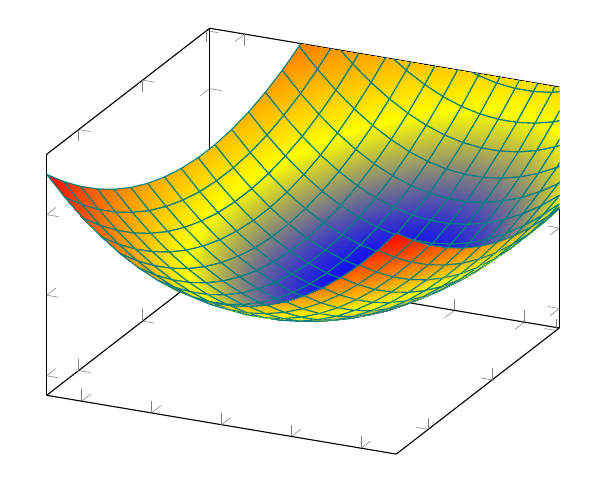
\begin{tikzpicture}
		
		\begin{axis}[scale=0.95 ,name=Ax1,ymax=0.99,xticklabels={\empty},yticklabels={\empty},zticklabels={\empty}]
			
			\addplot3 [
			domain=-50:50,
			domain y = -50:50,
			samples = 20,
			samples y = 20,
			surf,
			shader = faceted interp,
			faceted color = teal] {x^2+y^2};
			
		\end{axis}

		
	\end{tikzpicture}
\end{center}
\item $f(x,y)=x^2-y^2$. Level Sets $c=0\implies x=\pm y$, $c=1\implies x^2-y^2=1$, $c=-1\implies x^2-y^2=-1$
\vspace{1cm}

\begin{center}
	\begin{tikzpicture}
	\begin{axis}[scale=0.95,name=Ax1,ymax=0.99,xticklabels={\empty},yticklabels={\empty},zticklabels={\empty}]
		
		\addplot3 [
		domain=-5:5,
		domain y = -3:3,
		samples = 20,
		samples y = 8,
		surf,
		shader = faceted interp,
		faceted color = teal] {x^2-y^2};
		
	\end{axis}
	\begin{axis}[scale=0.95,name=Ax2,at={($(Ax1.north east)+(2cm,0)$)},anchor=north west,hide axis,xmin=-2,xmax=2,ymin=-2,ymax=2,restrict x to domain=-10:10]
		\addplot[blue, variable=t,domain=0:360,samples=200] ({sec(t)}, {tan(t)}) node[xshift=1cm, yshift=1cm]{$c=1$} node[xshift=0cm, yshift=2.5cm]{$c=-1$};
		\addplot[blue,variable=t,domain=0:360,samples=200] ({tan(t)}, {sec(t)});
		\addplot[blue]{x};
		\addplot[blue]{-x};
	\end{axis}
\end{tikzpicture}
\end{center}
\item $f(x,y)=xy$

$u=\frac{x+y}{\sqrt{2}},v=\frac{x-y}{\sqrt{2}}$. Then $x=\frac{u+v}{\sqrt{2}},y=\frac{u-v}{\sqrt{2}}$ and $f(x,y)=\frac{u^2-v^2}{2}$. Here $A=\frac12\lt[ \begin{matrix}
	0 &1\\ 1 &0
\end{matrix} \rt]$. Hence eigenvectors are $\lt[ \begin{matrix}
1\\ 1
\end{matrix} \rt]$ and $\lt[ \begin{matrix}
1\\ -1
\end{matrix} \rt]$

\begin{center}
	\begin{tikzpicture}
		\begin{axis}[scale=0.95,name=Ax1,ymax=0.99,xticklabels={\empty},yticklabels={\empty},zticklabels={\empty}]
			
			\addplot3 [
			domain=-5:5,
			domain y = -3:1,
			samples = 20,
			samples y = 8,
			surf,
			shader = faceted interp,
			faceted color = teal] {x*y};
			
		\end{axis}
		\begin{axis}[scale=0.95,name=Ax2,at={($(Ax1.north east)+(2cm,0)$)},anchor=north west,
			axis x line=center,
			axis y line=center,
			xlabel = $x$,
			ylabel = {$y$},
			ymax=3,
			ymin=-3,
			ticks=none,
			]
			\node[right] at (-2,2) {$C=-2$};
			\node[right] at (-0.7,0.2) {$C=0$};
			
			%Below the red is defined
			\addplot [
			domain=-2:-0.1, 
			samples=50, 
			color=red,
			]
			{1/x};
			\addplot [
			domain=0.1:2, 
			samples=50, 
			color=red,
			]
			{(1/x)};  
			\addplot [
			domain=-2:-0.1, 
			samples=50, 
			color=red,
			]
			{ -1/x};
			\addplot [
			domain=0.1:2, 
			samples=100, 
			color=red,
			]
			{(-1/x)};
			
			% Now the teal
			\addplot [
			domain=-2.:-0.1, 
			samples=50, 
			color=teal,
			]
			{(0.5/x)};
			\addplot [
			domain=0.1:2, 
			samples=50, 
			color=teal,
			]
			{(0.5/x)};
			\addplot [
			domain=-2:-0.1, 
			samples=100, 
			color=teal,
			]
			{ -0.5/x};   
			\addplot [
			domain=0.1:2, 
			samples=50, 
			color=teal,
			]
			{(-0.5/x)};
			
			%Here green  is defined
			\addplot [
			domain=-2:-0.1, 
			samples=50, 
			color=green,
			]
			{-2/x};
			\addplot [
			domain=-2:-0.1, 
			samples=50, 
			color=green,
			]
			{2/x};
			\addplot [
			domain=0.1:2, 
			samples=50, 
			color=green,
			]
			{-2/x};
			\addplot [
			domain=0.1:2, 
			samples=50, 
			color=green,
			]
			{-2/x};
			
		\end{axis}
	\end{tikzpicture}
\end{center}
\end{enumerate}

We should understand graphs of `Quadratic Hypersurfaces' $\Phi(x)=0$, where $\Phi(x)$ is  a quadratic polynomial in $n$ variables. 

`Standard Form' is $\lm_1x_2^2+\lm_2x_2^2+\cdots+\lm_nx_n^2+$ Constant. We will see that by a shift of origin and orthogonal change of coordinates, we can express any general quadratic $\Phi$ to the Standard Form
\begin{enumerate}[label=\bfseries\tiny\protect\circled{\small\arabic*}]
	\item Getting Rid of Linear Part
	
	\begin{align*}
		& \lm_1x_1^2+\lm_2x_2^2+\cdots+\lm_nx_n^2+p_1x_1+\cdots+p_nx_n+\text{ constant}\\
		= & \lm_1(x_1-a_1)^2+\cdots+\lm_n(x_n-a_n)^2+\text{ another constant} \quad [-2\lm_ia_i=p_i\implies a_i=-\frac{p_i}{2\lm_i},\text{ assuming }\lm_i\neq 0]
	\end{align*}
\item In general we express $x$ in terms of new basis consisting of orthonormal eigenvectors of $A$. 

Nationalizing a matrix $A$, $\Gamma^{-1}A\Gamma=D $-diagonal matrix where columns of $\Gamma=$ eigen basis corresponding to matrix $A$. Here $\Gamma$ is orthogonal matrix $\Gamma\Gamma^T=\Gamma^T\Gamma=I$ and we have $\Gamma^TA\Gamma=D\implies A=\Gamma D\Gamma^T$. Now $$\Phi(x)=x^TAx+pX+r$$Let $x^*=$ coordinate vector of $x$ in terms of  new basis consisting of columns of $\Gamma$\begin{align*}
	x^* & = \Gamma^{-1}x=\Gamma^T x \text{ we use this to formulate }\Phi\\
	& = (x^T\Gamma)D(\Gamma^Tx)+p\Gamma(\Gamma^Tx)+r=\Phi(x)\\
	& = \underset{  \substack{  \downarrow \\ \text{standard} \\ \text{form}  }  }{{x^*}^TDx^*}+\underset{\substack{\downarrow \\ \text{linear} \\ \text{form}  }  }{p\Gamma x^*}+r=\Psi(x^*)
\end{align*} Use step 1 to eliminate the linear term
\end{enumerate}

Now we will look into some more examples.
\begin{enumerate}[label=\bfseries\tiny\protect\circled{\small\arabic*}]
	\item $f(x,y)=x^2-xy+y^2$
	
	$$A=\lt[ \begin{matrix}
		1 & -\frac12\\ -\frac12 & 1
	\end{matrix} \rt]\text{ and }H=\lt[ \begin{matrix}
	1 & -1\\ -1 & 2
\end{matrix} \rt]$$ $H$ is  positive definite because diagonal entries are positive and determinant $ =3>0$. So the unique critical point $(0,0)$ is a local minima
\nt{
$2\times 2$ symmetric matrix $\lt[ \begin{matrix}
	a & c\\ c& b
\end{matrix} \rt]$ is positive definite $\iff \begin{cases}
a,b>0\\ ab-c^2>0
\end{cases}$
}

\item $\Phi(x)=2x^2+3y^2-4xy-12x-14y+21=\mat{x\\y}^TA\mat{x\\ y}+p\mat{x\\ y}+r$

$$A=\mat{2& -2\\ -2 & 3}\text{ and }H=\mat{4 & -4\\ -4 & 6}\text{ and }p=\mat{ -12 & 14}$$ $H$ is positive definite as diagonal entries are positive and determinant $=8>0$. The critical point is the solution of the equation $$H\mat{x\\ y} = - \mat{ -12 \\ 13} \iff \mat{4 & -4\\ -4 & 6}\mat{x\\ y}=-\mat{-12\\ 14}$$Hence $x=2$, $y=-1$. Therefore minimum value $\Phi(2,-1)=2$
\nt{
Another way: Complete the squares \begin{align*}
	\Phi(x) & = 2(x-2)^2+4(y+1)^2-4(x-2)(y+1)+2\\
	& = 2u^2+3v^2-4uv+2
\end{align*}}
\item $f(x,y)=x^3+y^3-3x-3y$

$$f'(x,y)=\mat{3x^2-3 & 3y^2-3}, \qquad \nabla f=\mat{3x^2-3\\ 3y^2-3}$$Critical points are $(x,y)$ such that $f'(x,y)=0$ i.e. $\begin{cases}
	3x^2-3=0\\ 3y^2-3=0
\end{cases}$. There are 4 critical points $=(\pm 1, \pm 1)$ $$\text{Hessian }H=\mat{6x & 0\\ 0 & 6x}$$ \begin{center}
\begin{tabular}{l}
	$(1,1,)\to$ local min, 	$(-1,-1)\to$ local max, $(\pm 1,\mp 1)\to$ saddle points
\end{tabular}
\end{center}
 \end{enumerate}
\nt{For $x^3-y^2+3x-3y$ there are no critical points}